% !Mode:: "TeX:UTF-8"
\documentclass[openany]{book}
% !Mode:: "TeX:UTF-8"
\usepackage[english]{babel}
\usepackage[UTF8]{ctex}
\usepackage{amsmath, amsthm, amssymb}

% Figure
\usepackage{graphicx}
\usepackage{float} %% H can fix the location
\usepackage{caption}
\usepackage[format=hang,singlelinecheck=0,font={sf,small},labelfont=bf]{subfig}
\usepackage[noabbrev]{cleveref}
\captionsetup[subfigure]{subrefformat=simple,labelformat=simple,listofformat=subsimple}
\renewcommand\thesubfigure{(\alph{subfigure})}

\usepackage{epstopdf} %% convert eps to pdf
\DeclareGraphicsExtensions{.eps,.mps,.pdf,.jpg,.png} %% bmp, gif not supported
\DeclareGraphicsRule{*}{eps}{*}{}
\graphicspath{{img/}{figure/}{../figure/}} %% fig directorys

%% \usepackage{pstricks} %% a set of macros that allow the inclusion of PostScript drawings directly inside TeX or LaTeX code
%% \usepackage{wrapfig} %% Wrapping text around figures

% Table
\usepackage{booktabs} %% allow the use of \toprule, \midrule, and \bottomrule
\usepackage{tabularx}
\usepackage{multirow}
\usepackage{colortbl}
\usepackage{longtable}
\usepackage{supertabular}

\usepackage[colorinlistoftodos]{todonotes}

% Geometry
\usepackage[paper=a4paper, top=1.5cm, bottom=1.5cm, left=1cm, right=1cm]{geometry}
%% \usepackage[paper=a4paper, top=2.54cm, bottom=2.54cm, left=3.18cm, right=3.18cm]{geometry} %% ms word
%% \usepackage[top=0.1cm, bottom=0.1cm, left=0.1cm, right=0.1cm, paperwidth=9cm, paperheight=11.7cm]{geometry} %% kindle

% Code
%% \usepackage{alltt} %% \textbf can be used in alltt, but not in verbatim

\usepackage{listings}
\lstset{
    backgroundcolor=\color{white},
    columns=flexible,
    breakatwhitespace=false,
    breaklines=true,
    captionpos=tt,
    frame=single, %% Frame: show a box around, possible values are: none|leftline|topline|bottomline|lines|single|shadowbox
    numbers=left, %% possible values are: left, right, none
    numbersep=5pt,
    showspaces=false,
    showstringspaces=false,
    showtabs=false,
    stepnumber=1, %% interval of lines to display the line number
    rulecolor=\color{black},
    tabsize=2,
    texcl=true,
    title=\lstname,
    escapeinside={\%*}{*)},
    extendedchars=false,
    mathescape=true,
    xleftmargin=3em,
    xrightmargin=3em,
    numberstyle=\color{gray},
    keywordstyle=\color{blue},
    commentstyle=\color{green},
    stringstyle=\color{red},
}

% Reference
%% \bibliographystyle{plain} % reference style

% Color
\usepackage[colorlinks, linkcolor=blue, anchorcolor=red, citecolor=green, CJKbookmarks=true]{hyperref}
\usepackage{color}
\def\red#1{\textcolor[rgb]{1.00,0.00,0.00}{#1}}
\newcommand\warning[1]{\red{#1}}

% Other
%% \usepackage{fixltx2e} %% for use of \textsubscript
%% \usepackage{dirtree}  %% directory structure, like the result of command tree in bash shell

   %导入需要用到的package
% !Mode:: "TeX:UTF-8"

% Chapter
%% \makeatletter\@addtoreset{chapter}{part}\makeatother %% have chapters numbered without interruption (numbering through parts)

% Equation
\makeatletter\@addtoreset{equation}{section}\makeatother 
\renewcommand\theequation{%
\thepart\arabic{chapter}%
-\thepart\arabic{section}%
-\thepart\arabic{equation}%
}

% Theorem
\newtheorem{definition}{D\'efintion}
\newtheorem*{thmwn}{Thm}
\newtheorem{theorem}{Th\'eor\`eme}[chapter]
\newtheorem{corollary}{Corollary}[theorem]
\newtheorem{lemma}{Lemma}
\newtheorem{proposition}{Proposition}[chapter]
\newtheorem*{attention}{Attention}
\newtheorem*{note}{Note}
\newtheorem*{remark}{Remark}
\newtheorem{example}{Example}
\newtheorem{question}{Question}[chapter]
\newtheorem{problem}{Problem}
\newtheorem*{answer}{Answer}
\newtheorem{fact}{Fact}

   %导入需要用到的package

\begin{document}
\title{Paper Reading Notes}
\author{Eric}
\maketitle
\tableofcontents
\frontmatter

\part{Computer}
M/M/1排队模型(M/M/1 model)是一种单一服务器(single-server)的(排队模型),可用作模拟不少系统的运作.
依据开恩特罗符号必须有下列的条件:
\begin{itemize}
\item 到达时间服从泊松分布(Poisson distribution)\ref{sec.distribution.poisson},
\item 服务时间是指数分布(exponentially distributed)\ref{sec.distribution.exponential},
\item 只有一部服务器(server)
\item 队列长度无限制
\item 可加入队列的人数为无限
\end{itemize}
\begin{figure}[htbp]
  \centering
  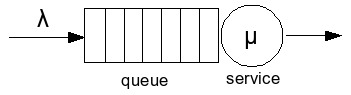
\includegraphics[scale = 0.3]{Mm1}\\
  \caption{Mm1}\label{fig.Mm1}
\end{figure}

这种模型是一种出生-死亡过程,此随机过程中的每一个状态代表模型中人数的数目.因为模型的队列长度无限且参与人数亦无限,故此状态数目亦为无限.例如状态0表示模型闲置,状态1表示模型有一人在接受服务,状态2表示模型有二人(一人正接受服务,一人在等候),如此类推. 此模型中,出生率(即加入队列的速率)$\lambda$ 在各状态中均相同,死亡率(即完成服务离开队列的速率)$\mu$亦在各状态中相同(除了状态0,因其不可能有人离开队列).

故此,在任何状态下,只有两种事情可能发生:
\begin{itemize}
\item 有人加入队列.如果模型在状态k,它会以速率$\lambda$ 进入状态$k + 1$
\item 有人离开队列.如果模型在状态k(k不等于0),它会以速率$\mu$进入状态$k ? 1$
\end{itemize}
%% %% on the state space {0,1,2,3,...}. This is the same continuous time Markov chain as in a birth–death process. The state space diagram for this chain is as below.
\begin{tikzpicture}%[->,>=stealth',shorten >=1pt,auto,node distance=2cm,semithick]
  % \tikzstyle{every state}=[fill=white,draw=black,text=black,minimum size=1.1cm]
  \tikzstyle{state}=[fill=white,draw=black,text=black,minimum size=1.1cm]
 
  \node[state] (A) {0};
  \node[state] (B) [right of=A] {$1$};
  \node[state] (C) [right of=B] {$2$};
  \node[state] (D) [right of=C] {$3$};
  \node[minimum size=1cm] (E) [right of=D] {$\cdots$};
  \node[state] (F) [right of=E] {$n-1$};
  \node[state] (G) [right of=F] {$n$};
  \node[state] (H) [right of=G] {$n+1$};
  \node[minimum size=1cm] (I) [right of=H] {$\cdots$};
 
  \path (A) edge [bend left] node {$\lambda$} (B);
  \path (B) edge [bend left] node {$\mu$} (A);
  \path (B) edge [bend left] node {$\lambda$} (C);
  \path (C) edge [bend left] node {$\mu$} (B);
  \path (C) edge [bend left] node {$\lambda$} (D);
  \path (D) edge [bend left] node {$\mu$} (C);
  \path (D) edge [bend left] node {$\lambda$} (E);
  \path (E) edge [bend left] node {$\mu$} (D);
  \path (E) edge [bend left] node {$\lambda$} (F);
  \path (F) edge [bend left] node {$\mu$} (E);
  \path (F) edge [bend left] node {$\lambda$} (G);
  \path (G) edge [bend left] node {$\mu$} (F);
  \path (G) edge [bend left] node {$\lambda$} (H);
  \path (H) edge [bend left] node {$\mu$} (G);
  \path (H) edge [bend left] node {$\lambda$} (I);
  \path (I) edge [bend left] node {$\mu$} (H);
\end{tikzpicture}

\begin{figure}[htbp]
  \centering
  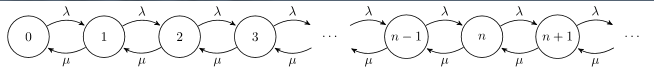
\includegraphics[scale = 0.5]{state_space}\\
  \caption{State space transmission}\label{fig.state_space}
\end{figure}

由此可见,模型的隐定条件为$\lambda < \mu$.如果死亡率小于出生率,则队列中的平均人数为无限大,故此这种系统没有平衡点.

此模型中有几项数值常被测量,例如:
\begin{itemize}
\item 一人在系统中的平均逗留时间
\item 一人在接受服务前的平均等候时间
\item 整个系统中的平均人数
\item 等候队列的平均人数
\item 一单位时间内系统完成服务人数,即服务速度
\end{itemize}

稳定状态下的公式

定义 $\scriptstyle \rho \,=\,{\tfrac  {\lambda }{\mu }}$.
则模型在状态i的机率为
$$
{\mbox{Prob}}(q=i)=\pi _{i}=(1-\rho )\rho ^{i}.\,
$$
由此,可给出各测量数值的公式:
整个系统的平均人数N:$\overline N={\frac  {\rho }{1-\rho }}$,
且其变异(variance)为$\sigma _{N}^{2}={\frac  {\rho }{(1-\rho )^{2}}}$.
一单位时间内系统完成服务的人数:$\overline N_{S}=\lambda \overline x=\rho$
在队列中等候服务的人数:$\overline N_{Q}={\frac  {\rho ^{2}}{1-\rho }}$
一人在系统中的平均逗留(等候+接受服务)时间:$T={\frac  {1}{\mu -\lambda }}$.
一人的平均等候时间:$W={\frac  {\overline N_{Q}}{\lambda }}=T-\overline x=T-{\frac  {1}{\mu }}={\frac  {\rho }{\mu -\lambda }}$

\begin{example}
可用M/M/1模型的例子众多,例如只有一位员工的邮局,只有一队列.客人进来,排队,接受服务,离开.如果客人进来的数目符合泊松过程,且服务时间是指数分布,则可用M/M/1模拟,并算出平均队列长度,不同等候时间的机率等.

M/M/1可一般化成为M/M/n模型,使可用时接受服务的人数为大于一.历史上,M/M/n模型首先被用来模拟电话系统,因为荷兰工程师Erlang发现客人打电话的速率符合泊松过程,且通话时间是指数分布,所以占用通讯线路的数目和等待接线的人数符合M/M/n模型.
\end{example}

%% ==============================================
%% ==============================================
\part{Math}
\chapter{概率论}
\label{sec:probability}

\section{指数分布(Exponential distribution)}
\label{sec.distribution.exponential}
一种\textbf{连续概率分布}.指数分布可以用来表示独立随机事件发生的时间间隔,比如旅客进机场的时间间隔,中文维基百科新条目出现的时间间隔等等.

\textbf{概率密度函数}
一个指数分布的概率密度函数是
$$f(x;\lambda )=\left\{{\begin{matrix}\lambda e^{{-\lambda x}}&,\;x\geq 0,\\0&,\;x<0.\end{matrix}}\right.$$
其中$\lambda  > 0$是分布的一个参数,常被称为率参数(rate parameter).即每单位时间发生该事件的次数.
指数分布的区间是$[0,\infty)$. 如果一个随机变量X 呈指数分布,则可以写作:$X \sim Exponential(\lambda )$.
$$
\int_0^{\infty} f(x)dx = 1
$$
\begin{figure}[htbp]
  \centering
  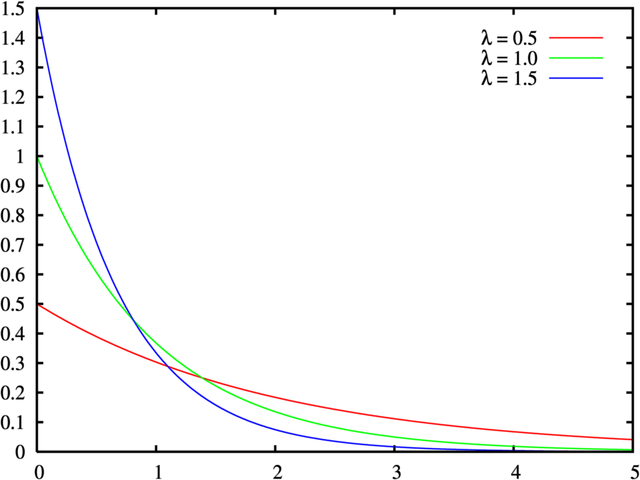
\includegraphics[scale = 0.3]{distribution_exponential}\\
  \caption{Exponential 概率密度函数}\label{fig.distribution.exponential}
\end{figure}
	
\textbf{累积分布函数}\\
累积分布函数可以写成:
$$F(x;\lambda )=\left\{{\begin{matrix}1-e^{{-\lambda x}}&,\;x\geq 0,\\0&,\;x<0.\end{matrix}}\right.$$
\begin{figure}[htbp]
  \centering
  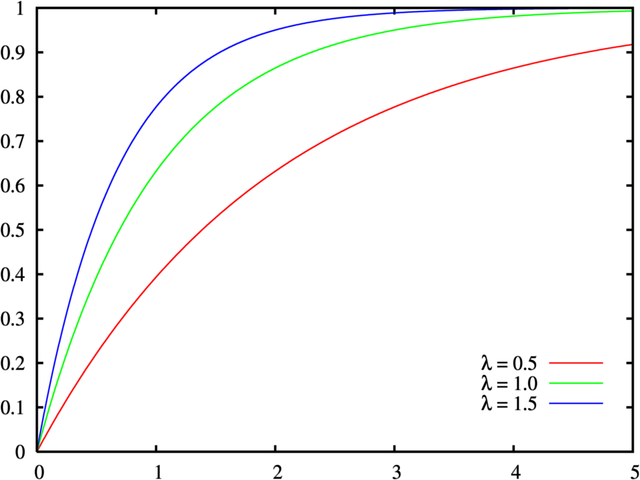
\includegraphics[scale = 0.3]{distribution_exponential_cdf}\\
  \caption{Exponential 累积分布函数}\label{fig.distribution.exponential.cdf}
\end{figure}
	
随机变量$X$ (概率参数是$\lambda$ ) 的期望值是:
$$
{\mathbf  {E}}[X]=\int_0^{\infty} xf(x)dx = {\frac  {1}{\lambda }}
$$
比方说:如果你平均每个小时接到2次电话,那么你预期等待每一次电话的时间是半个小时.
$X$ 的方差是:
$${\mathbf  {D}}[X]={\frac{1}{\lambda ^{2}}}
$$
$X$ 的偏离系数是: $V[X] = 1$

\textbf{与泊松过程的关系}\\
泊松过程是一种重要的随机过程.泊松过程中,第k次随机事件与第$k+1$次随机事件出现的时间间隔服从指数分布.这是因为,第$k$次随机事件之后长度为$t$的时间段内,第$k+1$次随机事件出现的概率等于$1$减去这个时间段内没有随机事件出现的概率.而根据泊松过程的定义,长度为$t$的时间段内没有随机事件出现的概率等于
$$
{\frac  {e^{{-\lambda t}}(\lambda t)^{0}}{0!}}=e^{{-\lambda t}}.
$$
所以第k次随机事件之后长度为t的时间段内,第$k+1$次随机事件出现的概率等于$1-e^{{-\lambda t}}$,这是指数分布.这还表明了泊松过程的无记忆性.

\section{Poisson分布}
\label{sec.distribution.poisson}
\textbf{离散分布}

泊松分布适合于描述单位时间内随机事件发生的次数的概率分布.如某一服务设施在一定时间内受到的服务请求的次数,电话交换机接到呼叫的次数,汽车站台的候客人数,机器出现的故障数,自然灾害发生的次数,DNA序列的变异数,放射性原子核的衰变数等等.

\bigskip
$X$ 表示在给定的时间间隔或指定区域$t$内结果的发生数量, 则泊松随机变量$X$的概率分布为:
$$
P(x,\lambda t)={\frac  {e^{-\lambda t}(\lambda t) ^{x}}{x!}}, \eqspace x=0,1,2,\cdots
$$
其中$\lambda$ 是单位时间(或单位面积)内随机事件的平均发生率,单位时间内得到结果的数量.
\begin{figure}[htbp]
  \centering
  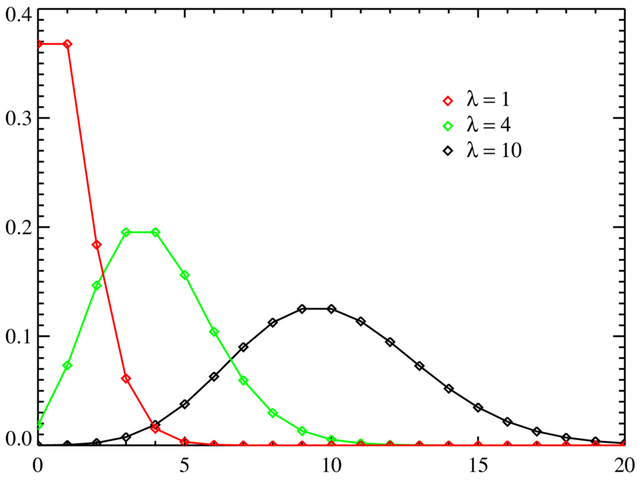
\includegraphics[scale = 0.3]{distribution_poisson}\\
  \caption{Poisson 概率分布}\label{fig.distribution.poisson}
\end{figure}

\begin{figure}[htbp]
  \centering
  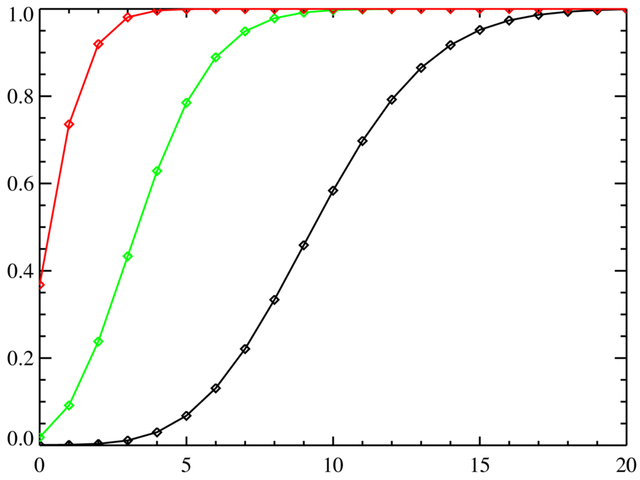
\includegraphics[scale = 0.3]{distribution_poisson_pmf}\\
  \caption{Poisson 累积分布函数}\label{fig.distribution.poisson.pmf}
\end{figure}

\begin{example}
一个试验中在$1 \mu s$ 内通过一计数器的平均辐射粒子数为4 个, 在某$1\mu s$ 中有6 个粒子通过计数器的概率为是多少?\\
根据参数, $x=6, \lambda t = 4 \times 1=4$, 得到
$$ p(6,4) = \frac{e^{-4} 4^6}{6!} = 0.1042 $$
\end{example}

\subsection{Features}	
\noindent
1.$E(X)=V(X)=\lambda$ \\
2.两个独立且服从泊松分布的随机变量,其和仍然服从泊松分布 (更精确地说:若$X \sim Poisson(\lambda_1)$且$Y \sim Poisson(\lambda_2)$,则 $X+Y \sim Poisson(\lambda_1+\lambda_2))$\\
3.与许多离散分布和连续分布一样, 随着均值越来越大, 泊松分布的形式越来越对称, 如图Figure~\ref{fig.distribution.poisson}.

\textbf{泊松过程的特点}
\begin{enumerate}
\item Les nombres d'occurrences dans des intervalles de temps disjoints sont ind\'ependants
\item La probabilit\'e d'une occurrence dans un petit intervalle de temps est proportionnelle \`a la longueur de cet intervalle, le coefficient de proportionnalit\'e \'etant$ \lambda$ 
\item La probabilit\'e qu'il y ait plus d'une occurrence dans un petit intervalle de temps est n\'egligeable
\end{enumerate}
Ces deux derni\`eres conditions forment la propri\'et\'e dite des \textbf{\'ev\'enements rares}.

Math\'ematiquement, ces propri\'et\'es se traduisent, si l'on note $(N_{t})_{{t\in {\mathbb  {R}}^{+}}}$ le processus de Poisson et ${\mathbb  {P}}$ la probabilit\'e, par:
\begin{enumerate}
\item $\forall t_{0}=0\leq t_{1}<\dots <t_{k}$, les variables al\'eatoires $(N_{{t_{k}}}-N_{{t_{{k-1}}}}),\dots (N_{{t_{1}}}-N_{{t_{0}}})$ sont ind\'ependantes
\item ${\mathbb{P}}(N_{{t+h}}-N_{t}=1)=\lambda h+o(h)$ lorsque $h\to 0+$ (t \'etant fix\'e)
\item ${\mathbb{P}}(N_{{t+h}}-N_{t}>1)=o(h)$ lorsque $h\to 0+$ (t \'etant fix\'e)
\end{enumerate}

\subsection{Poisson 分布与二项分布的关系}
%% http://my.oschina.net/u/347414/blog/129195
在二项分布的伯努利试验中,如果试验次数$n$很大,二项分布的概率$p$很小,且乘积$\lambda = n$ \\$p$比较适中,则事件出现的次数的概率可以用泊松分布来逼近.事实上,\textbf{二项分布可以看作泊松分布在离散时间上的对应物}.
\begin{proof}
证明如下.首先,回顾e的定义:
$$
\lim _{{n\to \infty }}\left(1-{\lambda  \over n}\right)^{n}=e^{{-\lambda }},
$$
二项分布的定义:
$$
P(X=k)={n \choose k}p^{k}(1-p)^{{n-k}}.
$$
如果令$p=\lambda /n$, $n$趋于无穷时$P$的极限:
$$
\begin{aligned}
\lim_{{n \to \infty }}P(X=k) & =\lim _{{n\to \infty }}{n \choose k}p^{k}(1-p)^{{n-k}}\\
& = \lim _{{n\to \infty }}{n! \over (n-k)!k!}\left({\lambda \over n}\right)^{k}\left(1-{\lambda \over n}\right)^{{n-k}}\\
& = \lim _{{n\to \infty }}\underbrace {\left[{\frac {n!}{n^{k}\left(n-k\right)!}}\right]}_{F}\left({\frac {\lambda ^{k}}{k!}}\right)\underbrace {\left(1-{\frac {\lambda }{n}}\right)^{n}}_{{\to \exp \left(-\lambda \right)}}\underbrace {\left(1-{\frac {\lambda }{n}}\right)^{{-k}}}_{{\to 1}}\\
& = \lim _{{n\to \infty }}\underbrace {\left[\left(1-{\frac {1}{n}}\right)\left(1-{\frac {2}{n}}\right)\ldots \left(1-{\frac {k-1}{n}}\right)\right]}_{{\to 1}}\left({\frac {\lambda ^{k}}{k!}}\right)\underbrace {\left(1-{\frac {\lambda }{n}}\right)^{n}}_{{\to \exp \left(-\lambda \right)}}\underbrace {\left(1-{\frac {\lambda }{n}}\right)^{{-k}}}_{{\to 1}}\\
& = \left({\frac {\lambda ^{k}}{k!}}\right)\exp \left(-\lambda \right)
\end{aligned}
$$
\end{proof}

\section{正态分布}
\textbf{连续概率分布}

若随机变量X服从一个位置参数为$\mu$ ,尺度参数为$\sigma$ 的概率分布,记为:$X\sim N(\mu ,\sigma ^{2})$

则其概率密度函数为
$$f(x)=\frac{1}{\sigma {\sqrt  {2\pi }}} e^{{- \dfrac{(x-\mu )^{2}}{2\sigma ^{2}}}}$$

\subsection{中心极限定理}
正态分布有一个非常重要的性质:在特定条件下,大量统计独立的随机变量的平均值的分布趋于正态分布,这就是中心极限定理.中心极限定理的重要意义在于,根据这一定理的结论,其他概率分布可以用正态分布作为近似.

参数为$n$和$p$的二项分布,在$n$相当大而且$p$接近$0.5$时近似于正态分布(有的参考书建议仅在$np$与$n(1-p)$至少为5时才能使用这一近似).
近似正态分布平均数为$\mu =np$且方差为$\sigma ^{2}=np(1-p)$.

泊松分布带有参数$\lambda$ 当取样样本数很大时将近似正态分布$\lambda$ .
近似正态分布平均数为$\mu =\lambda$ 且方差为$\sigma ^{2}=\lambda$ .

这些近似值是否完全充分正确取决于使用者的使用需求.

\chapter{PCA: Principal component analysis}
a useful statistical technique

wiki: the frist principal component has the largest possible variance.\\
\noindent
用covariance matrix 矩阵来讲解的话, 说是最大的eigenvalue 对应的eigenvector所在方向为the most principal component方向

\section{Idea}
我们以二元变量$X = (X_1, X_2)$为例, 说明主成分分析的思想. 对此二维变量进行了$n$ 次观测, 得到数据$x_i = (x_{i1},x_{i2}) \eqspace (i=1,2,\dots,n))$.假设它们在二维平面x1ox2上的分布如Figure~\ref{fig.PCA.idea}所示
\begin{figure}[htbp]
  \centering
  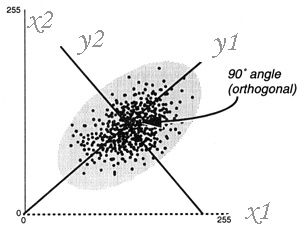
\includegraphics[scale = 0.7]{PCA_idea}\\
  \caption{PCA idea}\label{fig.PCA.idea}
\end{figure}
考虑如下一种极端情况,即$X_1$和$X_2$的相关系数的绝对值为$1$,则$(x(i_1),x(i_2))(i=1,2,...n)$以概率$1$分布在一条直线$L$上,若将原坐标系沿逆时针方向旋转一个角度$\theta $得到新的直角坐标系$y_1oy_2$,使坐标轴$oy_1$与$L$重合,这时观测点$(x(i_1),x(i_2))(i=1,2,...n)$则可由它们在$oy_1$上的坐标所决定,这些观测点在$oy_1$上的坐标为
$$ y(i_1)=x(i_1)cos\theta +x(i_2)sin\theta ,    i=1,2,...n $$
它们是原观测数据的线性组合且在$oy_1$轴上的分散性(即样本方差)达到最大. 这相当于对原变量$(X_1,X_2)$作适当的线性变换得新的变量$Y_1$,即
$$ Y_1=X_1cos\theta +X_2sin\theta , $$
其中$\theta $的选择使得$Var(Y_1)$最大且$Y_1$的相应观测值完全可以反映原二元变量$(X_1,X_2)$的观测值的分布状况. 一般情况下,将$ox_1$轴沿逆时针旋转到观测点具有最大分散性的方向$oy_1$上(观测点在$oy_1$轴上的投影到均值点的距离大于在$ox_1$上投影到均值点的距离),使该方向所含的数据间的差异的信息最多. 同样的,再旋转$ox_2$到$oy_2$. 我们将相应的变量
$$ Y_1=X_1cos\theta +X_2sin\theta , $$
$$ Y_2=X_1sin\theta +X_2cos\theta , $$
分别称为$X_1$和$X_2$的第一和第二主成分. 设想数据在$oy_2$方向上的分散性很小,因而用一元数据便可以反映二元数据的绝大部分信息,即达到了降维的目的. 
综上所述,主成分分析是研究如何通过少数几个主成分来解释多变量的方差-协方差结构的分析方法,也就是求出少数几个主成分(变量) ,使它们尽可能多地保留原始变量的信息,且彼此不相关. 它是一种变换方法,即把给定的一组变量通过线性变换,转换为一组不相关的变量,在这种变换中,\textbf{保持变量的总方差不变},同时具有最大方差,称为第一主成分;具有次大方差,称为第二主成分. 依次类推. 

find application in face recognition and image compression, and is a common technique for finding patterns in data of high dimension.

\section{总体主成分的定义}
设$\vecteur{X}$ 为某实际问题涉及的n 个随机变量, 记$\mathrm{X} = \vecteur{X}^t$, 其协方差矩阵为
$$
\Sigma = (\sigma)_{n \times n} = E[(\mathrm{X} - E(\mathrm{X}))(\mathrm{X} - E(\mathrm{X}))^t]
$$
设$l_i = (l_{i1},l_{i2},\dots,l_{in})^t \eqspace (i=1,2,\dots,n)$, 考虑下列线性组合
$$
\left\{
  \begin{array}{ll}
	  Y_1 = l_1^t \mathrm{X} & = l_{11}X_1 + l_{12}X_2 + \cdots + l_{1n}X_n \\
	  Y_2 = l_2^t \mathrm{X} & = l_{21}X_1 + l_{22}X_2 + \cdots + l_{2n}X_n \\
		  \vdots\\
	  Y_n = l_n^t \mathrm{X} & = l_{n1}X_1 + l_{n2}X_2 + \cdots + l_{nn}X_n
  \end{array}
\right.
$$
有
$$
\begin{aligned}
E(Y_i)
& = E(l_i^t \mathrm{X}) \\
& = E(l_{i1}X_1 + l_{i2}X_2 + \cdots + l_{in}X_n) \\
& = l_{i}^t E(X)
\end{aligned}
$$
$$
\begin{aligned}
Cov(Y_i,Y_j)
& = E[(Y_i - E(Y_i))(Y_j - E(Y_j))^t] \\
& = E[(l_i^tX - l_i^tE(X_i))(l_j^tX - l_j^tE(X))^t] \\
& = E[l_i^t (X-E(X)) (X-E(X))^t l_j]\\
& = l_i^t E((X-E(X))(X-E(X))^t) l_j \\
& = l_i^t \Sigma l_j
\end{aligned}
$$
$$Var(Y_i) = Cov(Y_i,Y_i) = l_i^t \Sigma l_i$$

\section{求法}
$\Sigma$ 的特征值及相应的正交单位化向量分别为$\lambda_1 \geq \lambda_2 \geq \cdots \geq \lambda_n \geq 0$ and $e_i,e_2,\cdots,e_n$, 则$X$ 的第$i$ 个主成分为
$$ Y_i = e_i^t \mathrm{X} = e_{i1}X_i + e_{i2}X_2 + \cdots + e_{in}X_n, \eqspace i=1,2,\cdots,n $$
其中$e_i = (e_{i1}, e_{i2}, \cdots+ e_{in})^t $\\
这时易见
$$
\left\{
	\begin{array}{l}
		Var(Y_i) = e_i^t \Sigma e_i = \lambda_i e_i^t e_i = \lambda_i, \eqspace i = 1,2,\cdots,n\\
		Cov(Y_i,Y_k) = e_i^t \Sigma e_k = \lambda_k e_i^t e_k = 0, \eqspace i \neq k
	\end{array}
\right.
$$

\section{性质}
\subsection{主成分的协方差及总方差}
令 $P = \vecteur{e}$, 则$P$ 为一正交矩阵, 记 $Y=\vecteur{Y}^t$ 为主成分向量, 则 $Y=P^t X$, 且
$$
Cov(Y) = Cov(P^t X) = P^t \Sigma P = Diag \vecteur{\lambda}
$$
由此得到, 主成分的总方差为
$$
\sum_{i=1}^n Var(Y_i) = \sum_{i=1}^n \lambda_i = tr(P^t \sigma P) = tr(\Sigma) = \sum_{i=1}^n Var(X_i)
$$

\subsection{主成分$Y_i$与$X_j$的相关系数}
由于$Y=P^t X$, 故 $X=PY$, 从而
$$
\left\{
  \begin{array}{l}
		  X_j = e_{1j}Y_1 + e_{2j}Y_2 + \cdots + e_{nj}Y_n \\
		  Cov(Y_i,X_j) = \lambda_i e_{ij}
  \end{array}
\right.
$$
由此可得$Y_i$与$X_j$ 的相关系数为
$$
\rho_{Y_i,X_j} = \frac{Cov(Y_i,X_j)}{\sqrt{Var(Y_i)} \sqrt{Var(X_j)}} = \frac{\lambda_i e_{ij}}{\sqrt{\lambda_i} \sqrt{\sigma_{jj}}} = \frac{\sqrt{\lambda_i}}{\sigma_{jj}} e_{ij}
$$

\subsection{标准化变量的主成分}
为了避免不同的物理量的不同量纲对计算的权重的影响, 需要normaliser.\\
令 $X_i^* = \dfrac{X_i - \mu_i}{\sqrt{\sigma_{ii}}}$, where $\mu_i = E(X_i), \sigma_{ii} = Var(X_i)$

\section{样本主成分: 以统计学的方式讲解}
\subsection{Standard Deviation}
$$
s = \sqrt{\dfrac{\sum_{i=1}^n (X_i - \overline{X})^2}{n-1}}
$$
\textbf{Why are you using $n-1$ and not $n$?}\\
Well, the answer is a bit complicated, but in general, if your data set is a sample data set, 
ie. you have taken a subset of the real-world (like surveying $500$ people about the election) then you must use $n-1$ 
because it turns out that this gives you an answer that is closer to the standard deviation that would result if you had used the entire population, than if you'd used$n$.
If, however, you are not calculating the standard deviation for a sample, but for an entire population, then you should divide by $n$ instead of $n-1$.\\
For further information, refer to \href{http://mathcentral.uregina.ca/RR/database/RR.09.95/weston2.html}{when $n$ or $n-1$ in computing the standard deviation}

Standard deviation and variance only operate on 1 dimension.\\
Covariance is always measured between 2 dimensions. If you calculate the covariance between one dimension and itself, you get the variance
$$ \operatorname{Var}(X) = \operatorname{E}\left[(X - E(x))^2 \right] = \dfrac{\sum_{i=1}^n (X_i - \overline{X})^2}{n-1} $$
$$ \operatorname{Cov}(X,Y) = \operatorname{E}{\big[(X - \operatorname{E}[X])(Y - \operatorname{E}[Y])\big]} =  \dfrac{\sum_{i=1}^n (X_i - \overline{X})(Y_i - \overline{Y})}{n-1} $$

The exact value is not as important as it’s sign (ie. positive or negative).
\begin{itemize}
\item If the value is positive,then that indicates that both dimensions increase together.
\item If the value is negative, then as one dimension increases, the other decreases.
\item In the last case, if the covariance is zero, it indicates that the two dimensions are independent of each other.
\end{itemize}

\subsection{The covariance Matrix}
the covariance matrix $\Sigma$ is the matrix whose $(i, j)$ entry is the covariance
$$
\Sigma_{ij}
= \mathrm{cov}(X_i, X_j) = \mathrm{E}\begin{bmatrix}
(X_i - \mu_i)(X_j - \mu_j)
\end{bmatrix}
$$
where $\mu_i = \mathrm{E}(X_i)$ is the expected value of the ith entry in the vector X. In other words, we have

$$
\Sigma
= \begin{bmatrix}
 \mathrm{E}[(X_1 - \mu_1)(X_1 - \mu_1)] & \mathrm{E}[(X_1 - \mu_1)(X_2 - \mu_2)] & \cdots & \mathrm{E}[(X_1 - \mu_1)(X_n - \mu_n)] \\ \\
 \mathrm{E}[(X_2 - \mu_2)(X_1 - \mu_1)] & \mathrm{E}[(X_2 - \mu_2)(X_2 - \mu_2)] & \cdots & \mathrm{E}[(X_2 - \mu_2)(X_n - \mu_n)] \\ \\
 \vdots & \vdots & \ddots & \vdots \\ \\
 \mathrm{E}[(X_n - \mu_n)(X_1 - \mu_1)] & \mathrm{E}[(X_n - \mu_n)(X_2 - \mu_2)] & \cdots & \mathrm{E}[(X_n - \mu_n)(X_n - \mu_n)]
\end{bmatrix}.
$$
The inverse of this matrix, $\Sigma^{-1}$ is the inverse covariance matrix, also known as the concentration matrix or precision matrix

If you ever need to find the eigenvectors of a matrix in a program, just find a maths library that does it all for you.  A useful maths package, called newmat, is available at \href{http://webnz.com/robert/}{newmat}

\subsection{PCA 的求解过程}
\begin{enumerate}
\item Get some data
\item Subtract the mean
\item Calculate the covariance matrix
\item Calculate the unit eigenvectors and eigenvalues of the covariance matrix
\item Choosing components and forming a feature vector
\item Deriving the new data set
\end{enumerate}
\end{document}
